
\documentclass{standalone}

\usepackage{tikz} %Graphics
\usetikzlibrary{matrix}
\usepackage{amsmath}
\usetikzlibrary{shapes.geometric, arrows}


\tikzstyle{startstop} = [ draw=none, minimum width=1.5cm, minimum height=1cm, text centered]
\tikzstyle{process} = [rectangle, rounded corners, minimum width=1.0cm, minimum height=1.0cm, text centered, draw=black, fill=blue!30]
\tikzstyle{process_score} = [circle, minimum width=1.0cm, minimum height=1.0cm, text centered, draw=black, fill=blue!30]

\tikzstyle{arrow} = [thick,->,>=stealth]
\tikzstyle{arrow_back} = [thick,<-,>=stealth]

%\usetikzlibrary{...}
\begin{document}
	\begin{tikzpicture}[node distance=2.6cm]	
		\node (A) {
			\begin{tikzpicture}[every node/.style={anchor=base,
				text height=.8em,text depth=.2em,minimum size=7mm}]
			    \matrix[fill=blue!30, 		    
			            matrix of nodes, 
			            nodes={draw,minimum size=1cm}, 
			            nodes in empty cells,
			            column sep=-\pgflinewidth,
			            row sep=-\pgflinewidth]
			    (M)
			    {
					$s^{f_1}_{i, 11}$   &   $...$   &   $s^{f_1}_{i, 1w}$  \\
					$...$   &   $...$   &   $...$  \\
					$s^{f_1}_{i, h1}$   &   $...$   &   $s^{f_1}_{i, hw}$ \\
				};
			\end{tikzpicture}
		};

		\node (B)[startstop, below of=A]{$(...)$};

		\node (C)[below of=B] {
	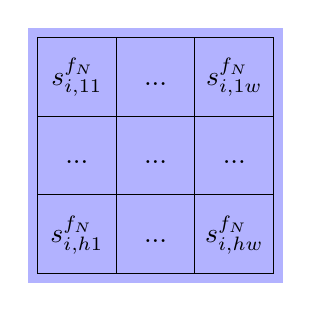
\begin{tikzpicture}[every node/.style={anchor=base,
		text height=.8em,text depth=.2em,minimum size=7mm}]
	\matrix[fill=blue!30, 		    
	matrix of nodes, 
	nodes={draw,minimum size=1cm}, 
	nodes in empty cells,
	column sep=-\pgflinewidth,
	row sep=-\pgflinewidth]
	(M)
	{
		$s^{f_N}_{i, 11}$   &   $...$   &   $s^{f_N}_{i, 1w}$  \\
		$...$   &   $...$   &   $...$  \\
		$s^{f_N}_{i, h1}$   &   $...$   &   $s^{f_N}_{i, hw}$ \\
	};
	\end{tikzpicture}
};
		\node (score_calc) [process_score, right of=B] {$+$};

		\node (so) [startstop, right of=score_calc] {$S_o = \lambda_o a_o$};
		\node(sk) [startstop, below of=score_calc] {$S_k = \lambda_o b$};
		
		\draw [arrow_back] (A) -- (score_calc);
		\draw [arrow_back] (B) -- (score_calc);
		\draw [arrow_back] (C) -- (score_calc);
		\draw [arrow_back] (score_calc) -- (so);
		\draw [arrow] (score_calc) -- (sk);
		\node[scale=1.5,text width=5cm, anchor=west, right] at (3.5,-1)
		{$s_{i,hw}^{f_k} = \overset{\lambda_i}{\overbrace{\lambda_o \omega_{hw}^{f_k}}} a_{i,hw}^{f_k}$};
	\end{tikzpicture}
\end{document}
